\documentclass[11pt,a4paper]{extarticle}
\usepackage[utf8]{inputenc}
\usepackage[spanish]{babel}
\usepackage{amsmath}
\usepackage{amsfonts}
\usepackage{amssymb}
\usepackage{graphicx}
\usepackage[left=1.2cm,right=1.2cm,top=2cm,bottom=2cm]{geometry}
\date{\small{\today}}
\usepackage{fancyhdr}
\usepackage{afterpage}
\usepackage{titlesec}
\usepackage{float}
\usepackage{gensymb}
\usepackage{xfrac}
\usepackage{tabularx}
\usepackage{multicol}
\usepackage[font=small]{caption}
\usepackage{scrextend}
\usepackage[toc,page]{appendix}

\renewcommand\appendixpagename{Apéndices}
\renewcommand\appendixname{Apéndice}

\titleformat{\section}{\Large\bfseries}{}{0em}{}[]
\titleformat{\subsection}{\large\bfseries}{}{0em}{}[]
\titleformat{\subsubsection}{\bfseries}{}{0em}{}[]
\titleformat{\chapter}{\large\bfseries}{}{0em}{}[]


\setlength\parindent{0pt}


\begin{document}
\title{Medición de Impedancias con Amplificador Lock In}
	\LARGE{\textsc{Laboratorio II}}\\
	\Large{Medición de Impedancias con Amplificador Lock In}\\
\begin{large}
\small\textsc{Horst, Raúl Tomás}\\
\small\textsc{Roqueta, Matías Daniel}\\
\small{Centro Atómico Bariloche y Instituto Balseiro, Comisión Nacional de Energía Atómica}\\
\end{large}
\setcounter{page}{1}

\lhead{Laboratorio II}%Materia
\rhead{Medición de Impedancias con Amplificador Lock In}%Título 
\chead{}

\lfoot{R. Horst, M. Roqueta}
\cfoot{Instituto Balseiro} 
\rfoot{\thepage} 
\renewcommand{\headrulewidth}{0.4pt} 
\renewcommand{\footrulewidth}{0.4pt} 
\pagestyle{fancy}

\hrule
\begin{multicols}{2}
\normalsize
\section{Resumen}

\section{Introducción}

\begin{figure}[H]
	\centering
	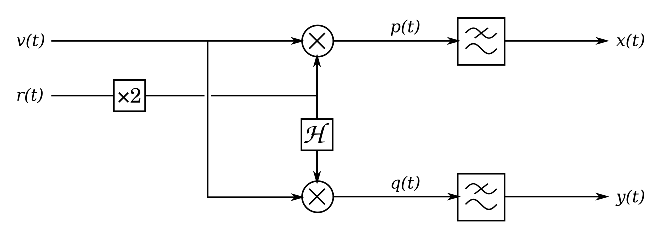
\includegraphics[width=\linewidth]{Images/lockin.eps}
	\caption{es un lockin}
	\label{fig:lockin}
\end{figure}


En la figura \ref{fig:lockin} hay un lockin

\section{Método Experimental}


\section{Resultados}

\section{Discusión}

\section{Conclusiones}

\bibliography{Antenas}
\bibliographystyle{ieeetr}

\end{multicols}
\newpage
\begin{appendices}
\vspace{-1em}
\hrule
\vspace{1em}
\normalsize
\section{Apéndice 1 - si pinta meter un apéndice}
\end{appendices}

\end{document}
